% \documentclass[11pt,a4paper]{article}
\documentclass[journal]{IEEEtran}

\usepackage[utf8]{inputenc}
\usepackage{mathrsfs,amsmath}
\usepackage{enumitem}
\usepackage{bigints}
\usepackage{indentfirst}
\usepackage{graphicx}
\usepackage{listings}
\usepackage{comment}
\usepackage{amsfonts}
\usepackage{float}
\usepackage{hyperref}
\usepackage{caption}
\graphicspath{ {./images/} }
\usepackage[section]{placeins}

\newenvironment{mathenum}[1][]{
\enumerate[#1]\mtmathitem}{$\endlist} 

\title {Support Vector Machines - Binary Classification \\[1ex] \large Project Report}
\author{Taha Adeel Mohammed  {\small CS20BTECH11052}, Shambhu Kavir {\small CS20BTECH11045}  }


\begin{document}

\maketitle

\begin{abstract} \it{
    Support Vector Machines (SVMs) are a supervised machine learning technique utilized for classification and regression analysis. It can be viewed as a convex optimization problem, where the goal is to find the hyperplane which maximizes the margin between the two classes of data points. In the case of non-linearly separable data, we introduce the concept of slack variables(error) to allow for some misclassification (soft-margin SVM). In this report, we will be focusing on the theory of SVMs and analysis of the underlying convex optimisation problems. We also implement the SVM algorithm from scratch using the CVXPY library and apply it to our sample dataset.
}
\end{abstract}

\section{\textbf{Origin of the Problem}}
The basic idea of any (Supervised) Machine Learning model is to predict a certain output 'y' for an input 'x' correctly, when a certain amount of training data is given. 
\hbadness=10000
\newline

For our classification problem, given a set of vectors $(\vec{x_1}, \vec{x_2}, ..., \vec{x_m})$, where $\vec{x_i} \in \mathbb{R}^n$, and a set of labels ($y_1, y_2, ..., y_m$), we need to find a function $f$ such that $f(\vec{x_i}) = y_i$ for all $i = 1, 2, ..., m$. \hbadness=10000
\newline


The SVM tries to solve this problem by assuming $f$ to be a separating hyperplane (assuming the input is linearly separable). It operates on the binary classification problem class, i.e., each $y_i$ can be either -1 or 1. More specifically, the SVM tries to find a plane: $\vec{w}^T\vec{x} + b = 0$ such that
\begin{align}
    f(\vec{x_i}) =
    \begin{cases}
        \,\;\;1 \quad   &\text{if }\; \vec{w}^T\vec{x_i} + b \geq 0 \\
        -1      \quad   &\text{if }\; \vec{w}^T\vec{x_i} + b < 0
    \end{cases}
\end{align}


% To evaluate the performance of the model, we define the \textbf{training error} as the mean of absolute errors of all the points in the dataset. This is called the \textbf{Training Risk} of the model. It is denoted by $R_{train}(f)$ and is given by:-
% \begin{align}
%     R_{train}(f) = \frac{1}{m}\sum_{i=1}^{m} \lvert\Vec{y}_i  - f(\Vec{x}_i) \rvert
% \end{align}

% We make an assumption in our model that the points in the dataset are selected from a set of independent and identically distributed random variables(i.i.d). Using the law of large numbers, we cam say that the expectation value of the training error is approximately equal to the testing risk. Hence for a good generalizable model, we need to minimize the training risk.
% \begin{align}
%     \mathbb{E}\left[ \lvert \textit{y} - \textit{f}(\vec{x}) \rvert  \right] \approx R_{train}(f) = \frac{1}{m}\sum_{i=1}^{m} \lvert\Vec{y}_i  - \textit{f}(\Vec{x}_i) \rvert
% \end{align}

We can theoretically find a separating hyperplane by solving the following feasaibility problem:
% \begin{align}
%     y_i(w^T x_i + b_i) > 0 , \forall i = 1, 2, ..., m
% \end{align}
% A strict inequality constraint is not practically implementable on CVXY or another solvers as aresult the solver converts a strict inequality to a non-strict one like this:
\begin{align*}
    y_i(\vec{w}^T \vec{x_i} + b_i) \geq 0, \forall \; i = 1, 2, ..., m
\end{align*}

The problem with setting the following constraints is that the values $\vec{w}, b = (\vec{0}, 0) $ statisfy the constraints and the solver will return these value to us. This will yield $(\vec{w}, b) = (\vec{0}, 0) $.\\

% The Linearly Separable Case
However, for linearly separable data, since a non-trivial solution $(\vec{w}, b)$ exists, $(k \vec{w}, k b)$ would also be a solution for any $k > 0$. Hence we can update our constraints to the following without affecting the existence or validity of the solution:
\begin{align*}
    y_i(\vec{w}^T \vec{x_i} + b_i) \geq 1, \forall \; i = 1, 2, ..., m
\end{align*}

To remove the redundancy of multiple solutions, we can add the following constraint:
\begin{align*}
    \min_{i = 1...m} \lvert \vec{w}.\vec{x} + b \rvert = 1
\end{align*}

Continuing from the above normalisation, we will get two hyperplanes, as show in Fig. \ref{fig:margin},  such that (for some $i,j$):
\begin{align*}
    \vec{w}.\vec{x_i} + b &= \;\;\,1 \\
    \vec{w}.\vec{x_j} + b &= -1
\end{align*}

\begin{figure}
    \centering
    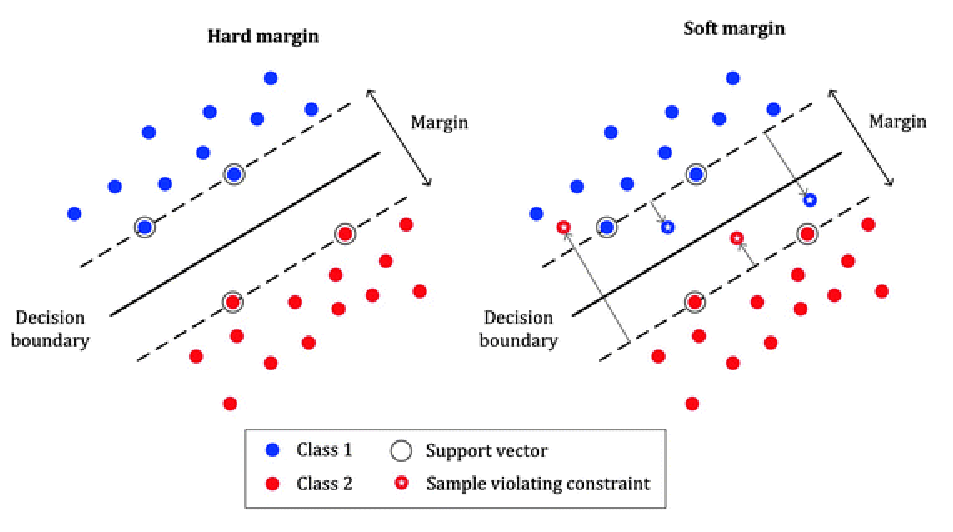
\includegraphics[width=0.4\textwidth]{margin.png}
    \caption{Hard-margin and soft-margin SVMs}
    \label{fig:margin}
\end{figure}

These are two parallel hyperplanes and the distance between them, called the \textbf{maximal margin} is given by
\begin{align}
   \text{maximal margin} = \frac{2}{\Vert {\vec{w} \Vert}  }
\end{align}


Now we frame our optimisation problem under the hypothesis that a
"good" classifier will maximise the ”margin” between the two
classes of data.
\begin{align}
    \vec{w}^* = \text{arg}\max_{\vec{w}, \;b}& \; \frac{2}{\Vert {\vec{w} \Vert}  } \\
    \text{s.t. } y_i(\vec{w}.\vec{x} + b) \geq 1, &\quad \forall\; i = 1...m \nonumber
\end{align}
This can also be framed as
\begin{align}
    \vec{w}^* = \text{arg}\min_{\vec{w}, b}&\; \frac{1}{2} \Vert {\vec{w} \Vert}^2 \\
    \text{s.t. } y_i(\vec{w}.\vec{x} + b) \geq 1, &\quad \forall\; i = 1...m \nonumber
\end{align}

The above \textbf{hard-margin SVM} is a \textbf{convex optimisation problem}, specifically,
a quadratic problem with linear constraints.\newline


In order to overcome the hurdle of linearly inseparable vectors, we allow some vectors to be misclassified by allowing some error $\xi_i$ for each vector $\vec{x_i}$. The new \textbf{convex optimisation problem} is called the \textbf{soft-margin SVM} problem and is given by
\begin{align}
    \vec{w}^* = \text{arg}\min_{\vec{w}, b}&\; \frac{1}{2} \Vert {\vec{w} \Vert}^2 + C \left( \sum_{i=1}^{m} \xi_i \right) ^ k\\
    \text{s.t. } y_i(\vec{w}.\vec{x} + b) \geq 1 - \xi_i, &\quad \forall\; i = 1...m \nonumber \\
    \xi_i \geq 0, &\quad \forall\; i = 1...m \nonumber
\end{align}


\section{\textbf{Analysis of the problem}}
\subsection{Hard-margin SVM}
The hard margin SVM convex optimization problem, as we've seen above, is given by
\begin{align}
    \vec{w}^* = \text{arg}\min_{\vec{w}, b}&\; \frac{1}{2} \Vert {\vec{w} \Vert}^2 \\
    \text{s.t. } y_i(\vec{w}.\vec{x} + b) \geq 1, &\quad \forall\; i = 1...m \nonumber
\end{align}

Now this can be solved using the Lagrangian method which is given by
\begin{align}
    L(\vec{w}, b, \vec{\lambda}) = \frac{1}{2} \Vert {\vec{w} \Vert}^2 - \sum_{i=1}^{m} \lambda_i (y_i(\vec{w}.\vec{x} + b) - 1)
\end{align}

Here $\lambda$ is the vector of non negative Lagrange multipliers. 
Differentiating the Lagrangian with respect to $\vec{w}$ and $b$ and equating to zero, we get
\begin{align}
    \frac{\partial L(\vec{w}, b, \vec{\lambda})}{\partial \vec{w}} &= \vec{w} - \sum_{i=1}^{m} \lambda_i y_i \vec{x}_i = 0 \\
    \frac{\partial L(\vec{w}, b, \vec{\lambda})}{\partial b} &= \sum_{i=1}^{m} \lambda_i y_i = 0
\end{align}
% Framing the dual problem using KKT conditions
We impose the condition $\vec{\lambda}.\vec{y} = 0$ and $\lambda_i \geq 0$  and substitute the value of $w$ to get the dual problem
\begin{align}
    \vec{\lambda}^* = &\text{ arg}\max_{\vec{\lambda}} \;\vec{\lambda}\cdot \vec{1} - \frac{1}{2} \vec{\lambda}^T D \vec{\lambda} \\
    &\text{s.t. } \vec{\lambda} \cdot \vec{y} = 0 \nonumber \\
    & \quad \vec{\lambda} \geq \vec{0} \nonumber \\
    \text{where } D_{ij} &= y_i y_j \vec{x}_i \cdot \vec{x}_j
\end{align}
% Meaning of the complementary slackness condition
The complementary slackness conditions are given by:-
\begin{align}
    \lambda_i (y_i(\vec{w}.\vec{x} + b) - 1) = 0, \forall i = 1...n
\end{align}
From the above equation, we can infer that the points in the dataset corresponding to $\lambda_i > 0$ are forced to be on the margin. These points are called the \textbf{support vectors}. The points corresponding to $\lambda_i = 0$ are not on the margin and do not affect the solution.


Once we solve the KKT conditions to obtain the values of the Lagrange multipliers $\vec{\lambda}$, the parameters of the hyperplane ($\vec{w^*}^T\vec{x} + b^* = 0$) can be obtained as
\begin{align}
    \vec{w}^* &= \sum_{i=1}^{m} \lambda_i^* y_i \vec{x}_i \\
    b^* &= y_i - \vec{w}^* \cdot \vec{x}_i
\end{align} 


\subsection{Soft-margin SVM}
% Framing the Soft Margin Classifier
We now consider the case when the data is not linearly separable. In such a case, we need to allow some points to be on the wrong side of the margin. We introduce a slack variable $\xi_i$ for each point in the dataset. The slack variable is the distance by which the point is on the wrong side of the margin. The optimisation problem is given by:-
\begin{align}
    \vec{w}^* = \text{arg}\min_{\vec{w}, b}&\; \frac{1}{2} \Vert {\vec{w} \Vert}^2 + C \left( \sum_{i=1}^{m} \xi_i \right) ^ k\\
    \text{s.t. } y_i(\vec{w}.\vec{x} + b) \geq 1 - \xi_i, &\quad \forall\; i = 1...m \nonumber \\
    \xi_i \geq 0, &\quad \forall\; i = 1...m \nonumber
\end{align}
Here we allow our classifier to commit $\xi_i$ error for sample $i$, but we penalize the total error using the addition of the second term in the objective function. We can control C and k so as to control how we want to penalize the error.

Therefore, the Lagrangian for the soft-margin problem is given by
\begin{align}
    L(\vec{w}, b, \vec{\lambda}, \vec{\mu}) = \frac{1}{2} \Vert \vec{w} \Vert^2 + C (\sum_{i=1}^{n} \xi_i)^k \notag \\
    \quad\quad- \sum_{i=1}^{n} \lambda_i (y_i(\vec{w} \cdot \vec{x} + b) - 1 + \xi_i) &- \sum_{i=1}^{n} \mu_i \xi_i
\end{align}

We need to minimize the Langrangian with respect to $\vec{w}, b, \xi_i$ and maximize it with respect to $\vec{\lambda}, \vec{\mu}$. Differentiating the Langarangian and equating to zero, we get
\begin{gather}
    \frac{\partial L(\vec{w}, b, \vec{\lambda}, \vec{\mu})}{\partial \vec{w}} = \vec{w} - \sum_{i=1}^{n} \lambda_i y_i \vec{x}_i = 0 \\
    \frac{\partial L(\vec{w}, b, \vec{\lambda}, \vec{\mu})}{\partial b} = \sum_{i=1}^{n} \lambda_i y_i = 0 \\
    \frac{\partial L(\vec{w}, b, \vec{\lambda}, \vec{\mu})}{\partial \xi_i} = Ck(\sum_{i=1}^{n} \xi_i)^{k-1} - \lambda_i - \mu_i = 0
\end{gather}

When $k > 1$, we have:-
\begin{align}
    \sum_{i=1}^{n} \xi_i = \left(\frac{\lambda_i + \mu_i}{kC}\right)^{\frac{1}{k-1}} 
\end{align}

Substituting these in the Lagrangian, we get  
\begin{align}
    L(\vec{\lambda}, \vec{\mu}) = \vec{\lambda}.\vec{1} - \frac{1}{2}\vec{\lambda}.D{\lambda}
\end{align}
From the above equation, we get the dual convex optimization problem as 
\begin{gather}
    \max_{\vec{\lambda}, \vec{\mu}} L(\vec{\lambda}, \vec{\mu}) = \vec{\lambda}\cdot\vec{1} - \frac{1}{2}\vec{\lambda}^T D\vec{\lambda} - \frac{(\mu_i + \lambda_i)^{\frac{k}{k-1}}}{(kC)^{\frac{1}{k-1}}} \left(1 - \frac{1}{k}\right) \nonumber \\
    \text{s.t. } \vec{\lambda} \geq 0, \quad \vec{\mu} \geq 0, \quad \vec{\lambda} \cdot \vec{y} = 0 \nonumber \\
    \text{where } D_{ij} = y_i y_j \vec{x}_i \cdot \vec{x}_j
\end{gather}

\section{\textbf{Code Implementation and Results}}
To implement the hard-margin and soft-margin SVM classifiers and solve the convex optimization problems, we use the \texttt{cvxpy} library in Python. To train the model, all dimensions of the input dataset are used. However, to visualize it, we use only the first two dimensions of the dataset and show the separating hyperplane.

\subsection*{Hard-margin SVM}
Below code snippet shows setting the optimization problem and constraints for the hard-margin SVM classifier, and then solving it using the \texttt{cvxpy} library.
\begin{figure}[H]
    \centering
    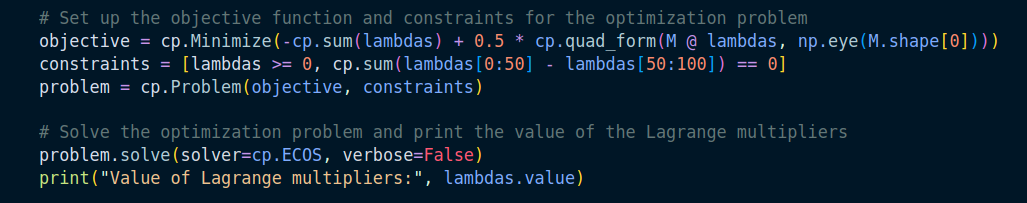
\includegraphics[width=0.48\textwidth]{code-snippet-hard.png}
    \caption{Code snippet for setting the optimization problem and constraints for the hard-margin SVM classifier}
    \label{fig:code1}
\end{figure}

It outputs the following result for our input dataset. We can see that the SVM classifier is able to separate the two classes perfectly.
\begin{figure}[!ht]
    \centering
    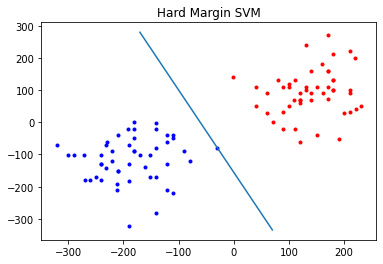
\includegraphics[width=0.4\textwidth]{hard-margin.png}
    \caption{Result of the hard-margin SVM classifier}
    \label{fig:res1}
\end{figure}


\subsection*{Soft-margin SVM}
The code for the soft-margin SVM classifier is similar to the hard-margin SVM classifier, except that we need to add the slack variables $\xi_i$ and the corresponding constraints. The code snippet for the same is shown below.
\begin{figure}[H]
    \centering
    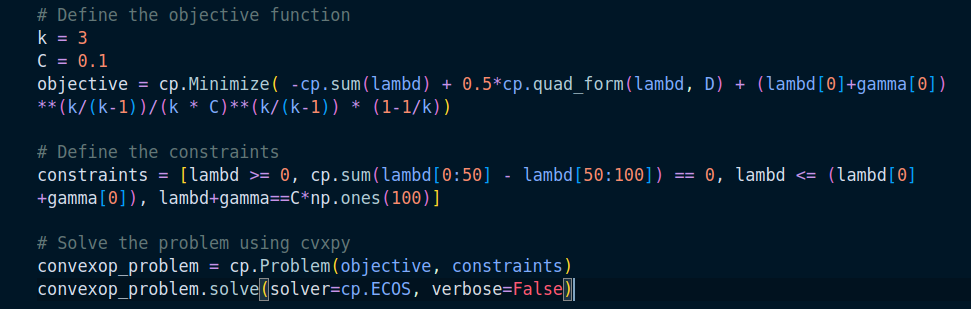
\includegraphics[width=0.48\textwidth]{code-snippet-soft.png}
    \caption{Code snippet for setting the optimization problem and constraints for the soft-margin SVM classifier}
    \label{fig:code2}
\end{figure}

\enlargethispage{-\baselineskip}
It outputs the following result for our input dataset. We can see that the soft-margin classifier is able to separate the two classes with very high accuracy. \vspace*{2cm}
\begin{figure}[!ht]
    \centering
    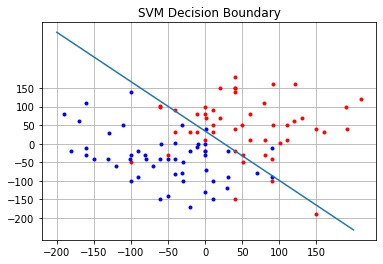
\includegraphics[width=0.4\textwidth]{soft-margin.png}
    \caption{Result of the soft-margin SVM classifier}
    \label{fig:res2}
\end{figure}

The results of our model on the test dataset are shown below. We can see that the our model computes values greater than 1 for most of the blue points, and less than -1 for most of the red points. Hence, it is able to classify the points correctly.
\begin{figure}[!ht]
    \centering
    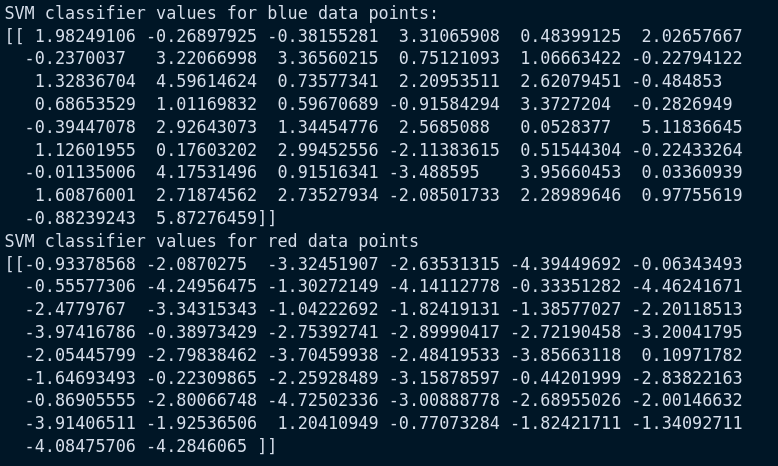
\includegraphics[width=0.4\textwidth]{result.png}
    \caption{Performance of the model}
    \label{fig:res3}
\end{figure}

\section{\textbf{Conclusion}}
\begin{itemize}
    \item In the field of machine learning, classification is one of the most fundamental tasks in data analysis. Therefore, hard and softt margin classifiers serve as a powerful tool for solving such problems.
    \item These classifiers aim to find the best hyperplane that can separate the input data into two different classifiers.
    \item This problem is interesting because it involves balancing two conflicting objectives:- maximizing the margin and minimizing the classification error.
    \item These classifiers have numerous applications such as image and speech recognition, text categorization, bioinformatics, etc.
    \item Further, this problem can be extended to handle non-linearly separable data using kernel methods. This involves mapping the input data to a higher dimensional space where it is linearly separable.
\end{itemize}


\pagebreak

\begin{thebibliography}{99}
    % Example reference 1
    \bibitem{ref1}
    \href{https://dspace.mit.edu/bitstream/handle/1721.1/9925/40121760-MIT.pdf?sequence=}{Support Vector Machines: Training and Applications} by Edgar E. Osuna, Robert Freund, and Federico Girosi, MIT, 1997.

    % Example reference 2
    \bibitem{ref2}
 \href{https://www.cs.huji.ac.il/~shais/UnderstandingMachineLearning/understanding-machine-learning-theory-algorithms.pdf}{Understanding Machine Learning: From Theory to Algorithms}, Shai Shalev-Shwartz and Shai Ben-David, Cambridge University Press, 2014.

 \bibitem{ref3}
 \href{https://courses.cs.vt.edu/cs5824/Fall15/pdfs/}{Machine Learning} Bert Huang, Virginia Tech, 2015.
    \bibitem{ref4}
    \href{https://web.stanford.edu/~boyd/cvxbook/bv_cvxbook.pdf}{Convex Optimization}, Stephen Boyd and Lieven Vandenberghe, Cambridge University Press, 2004.    
    \bibitem{ref5}
    \href{https://www.di.ens.fr/~mallat/papiers/svmtutorial.pdf}{A Tutorial on Support Vector Machines for Pattern Recognition}, Christopher J.C. Burges, Data Mining and Knowledge Discovery, 1998.

    % Add more references if needed...
\end{thebibliography}

\end{document}


